\minitoc

As detailed in the problem statement \ref{S_problem_statement}, one of the motivations of this thesis is to identify the methods to integrate usage control correctly in distributed ledgers, notably for performance issues (\hyperref[obj:23]{\emph{Objective 3}}). Indeed, adding the usage control system, or any privacy-enhancing technologies, to an existing distributed ledger creates additional bottlenecks. Firstly, the usage control system itself has performance limitations that sometimes exceed the ledger constraints. Besides, the interactions between the usage control system and the distributed ledger can create network or storage bottlenecks. Finally, the large number of devices in the Internet of Things creates significant network interactions between devices and the usage control system e.g., between the Policy Enforcement Points and the Policy Decision Point. This chapter focuses on the integration process. First, the existing integration schemes in the literature are introduced (Section \ref{S_state_of_the_art_ucon_dlt}). Then, we focus on identifying the most suitable technologies to integrate, as well as the purpose and methods of integration (Section \ref{S_integration_usage_control_with_dlt}). The integration process is evaluated to measure its performance benefits accurately (Section \ref{S_performance_evaluation}). A privacy threat assessment is also conducted in the general context of data trading, highlighting the benefits of usage control to preserve privacy (Section \ref{S_privacy_evaluation}), before concluding (Section \ref{S_conclusion_integration}).

\section{State-of-the-art usage control with distributed ledgers}
\label{S_state_of_the_art_ucon_dlt}

Integration of usage control with distributed ledgers, often referred to as \emph{incorporation}, has been proposed in the literature to benefit from distributed ledger properties. In particular, private blockchains are often leveraged for the following reasons:
\begin{itemize}
    \item \emph{auditability} and the possibility to monitor data while controlling data access simultaneously \cite{Khan2020, Ma2020};
    \item \emph{smart contracts} to enforce usage control and process data automatically \cite{Ma2020, Zhang2022}; 
    \item \emph{performance} with better network response time and low computation requirements \cite{Salimitari2020} in comparison with public blockchains.
\end{itemize}

Khan \emph{et al.}~\cite{Khan2020} incorporated the components of the UCON framework into the Hyperledger Composer, to form the BlockU model. The main reason stated by the authors is the continuous monitoring of the data access, thanks to attribute mutability. UCON is incorporated by using the Hyperledger Composer layer, a layer dedicated to modeling applications. Therefore, this incorporation can be seen as peripheral as the UCON components do not contribute to the blockchain network, and performance aspects are ignored. Besides, this work is not focused on IoT use cases.

Ma \emph{et al.}~\cite{Ma2020} proposed a decentralized usage control on both a public and a permissioned blockchain, respectively Ethereum and Hyperledger. A clear focus is given to privacy and decentralization to prevent accidental or intentional data leaks. All data operations are processed directly on the private blockchain with smart contracts, the degree of integration is consequently quite high. The public blockchain is used to introduce a reward mechanism, to encourage users to provide quality usage control data. However, the integration of usage control into the blockchain benefits usage control but not the blockchain network.

Shi \emph{et al.}~\cite{Shi2021} designed a Distributed Usage Control Enforcement (DUCE) solution for the Internet of Things, to tackle privacy issues related to the Cloud-Enabled Internet of Things (CEIoT). DUCE uses distributed PDP and PEP components and leverages private blockchains to store tamper-proof and traceable data on the ledger. The policies are written in the XACML language and then converted by an algorithm into the Solidity language for smart contracts. DUCE relies on a \emph{Trusted Environment Execution} (TEE) to enforce trustworthy processing of the rules.

Zhang \emph{et al.} \cite{Zhang2022} devised an efficient data trading scheme with usage control for Industrial IoT (IIoT). The scheme is based on Hyperledger Fabric and uses Intel SGX to define protected private regions of memory. Similarly to the above-mentioned related works, the authors utilize smart contracts to automatically trade data. To tackle usage control overhead on the data trading system, the authors rely on \emph{Policy Monitors} (PM) on the user side, using the SGX as a TEE. This enables the offloading usage policy enforcement on the user side, addressing scalability issues.

\section{Integration of usage control with distributed ledgers}
\label{S_integration_usage_control_with_dlt}

In this section, the principles of usage control integration with distributed ledger technologies are discussed. First, we propose criteria to determine if a technology is suitable for integration in Section~\ref{ss_integrability_criteria}. Then Section~\ref{ss_integration_benefits} details the different benefits of integration. 
Finally, Section~\ref{ss_integration_methodology} describes \sul{the method to integrate} usage control system with the distributed ledger technology.

\subsection{Integration suitability criteria}
\label{ss_integrability_criteria}


The distributed ledgers are heterogeneous because of diverse consensus methods, incentives, access control methods or even transaction graphs. To design a relevant integration scheme of usage control, it is first necessary to identify the requirements of this integration to find out the suitable distributed ledger technologies. Therefore, we propose a classification (cf. Table~\ref{tab:classification}) relying on three categories of features: the consensus method, the incentive to contribute to the network, and the graph of transactions. 

\textbf{Method of analysis.}
\begin{figure}[t]
\centering
 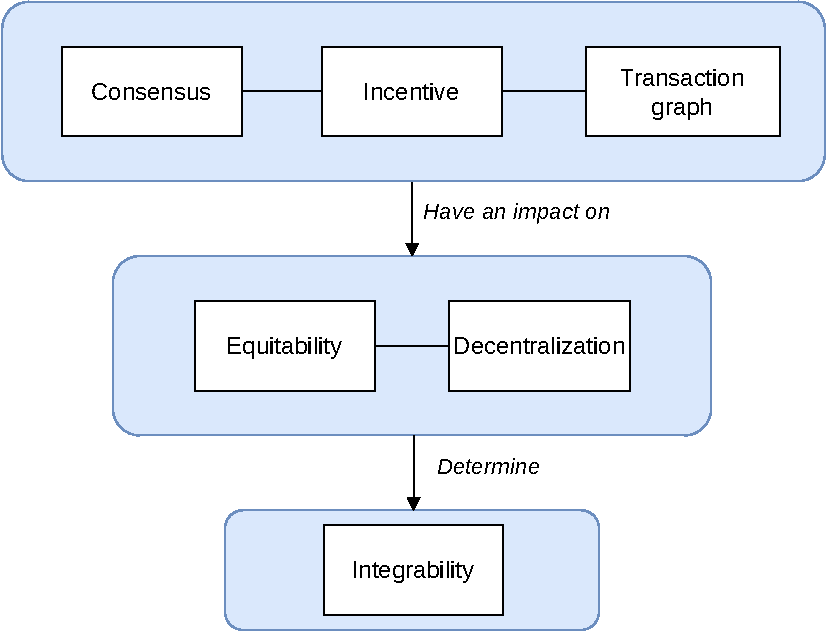
\includegraphics[scale=0.75]{Images/analysis.pdf}
\caption{Criteria used for integration suitability - schematized}
\label{F_analysis}
\end{figure}
To determine whether a DLT instance can integrate properly with the usage control system, we consider two properties of distributed ledger features: decentralization and equitability. These properties are directly influenced by other ledger features which are the basis of our analysis: 1) the consensus method; 2) the incentive to contribute to the network; 3) the transaction graph structure. The method of analysis is schematized in Figure \ref{F_analysis}.
\emph{Equitability} describes the possibility for every user to have a fair part in the decision-making and consensus processes. Particularly, it includes devices with poor computation or storage capacities. This property ensures small devices in the network have an actual impact, and that a small fraction of users do not monopolize the power in the network.
\emph{Decentralization}, besides providing performance and security benefits, is an interesting property to assess the integration suitability. Indeed, decentralization partially reflects the above-mentioned equitability. A fully decentralized network is likely to rely on local consensus to make decisions, which gives a bigger impact on participating devices~\cite{Popov2020, Steen2020}. %In contrast, centralization
Decentralization can take several forms, all expressing power asymmetries~\cite{Bodo2021}:  %. In distributed ledgers, centralization can take two forms~\cite{Bodo2021}: 
1) decentralization in the governance; 2) decentralization in terms of power, where nodes, or more likely node aggregates, have disproportionate power over the rest of the network. For instance, the proof of work consensus method gives power to the most powerful mining pools, while the proof of stake creates another form of centralized capital power. Highly centralized governance is often a prerequisite for a distributed network to work, which means a network can be highly centralized regarding only one centralization aspect, i.e., governance or power, but not the other. 
% The fairer and the more decentralized the network, the stronger the integration. 
The integration is more relevant as equitability and decentralization increase.
The distributed ledger features have an impact on these two properties of equitability and decentralization. To determine the characteristics that favor or hinder integration, three categories of features are next analyzed. 

\textbf{Consensus method.}
Consensus methods are very diverse, but the following are considered in our analysis:

\begin{itemize}
    \item \emph{Proof of Work}: due to computation concerns, a challenging computation race will exclude low-power devices from participating in the consensus. Even though the UCS could make a moderate profit while fulfilling its role, it is not an interesting application for our integration project; 
    \item  \emph{Proof of Stake}: PoS better fits the IoT computational requirements, but has several drawbacks for integration. First, a device can not contribute to the consensus unless it has a stake. Sensors in particular do not have the motivation or the possibility to hold a cryptocurrency asset, either for the consensus or to make transactions~\cite{Raghav2020}. The proof of stake also tends to centralize the network in the hands of a few users, either the delegates (DPoS) or the richest users. Equitability is therefore not achieved with this consensus method. Integrating the UCS in a distributed ledger based on PoS is not relevant, as devices can not contribute to the network;
    \item \emph{Proof of Authority}: PoA, contrary to the proof of stake, does not require holding a cryptocurrency asset. Nevertheless, PoA, by delegating the power to a few nodes considered trustworthy, limits the possibility to integrate the UCS components;
    \item \emph{Proof of Elapsed Time}: in PoET, miners are chosen at random using timers. This consensus method ensures equitability. In this setting, the components of the usage control system could contribute to the consensus, and integration is relevant. However, PoET is limited to private ledgers, as users must first join the network and gain a membership certificate to be allowed to start the timer; 
     \item \emph{Practical Byzantine Fault Tolerance}: all nodes take part in the voting process with equal power, providing the equitability property. Besides, this consensus method is suitable for the IoT but only on private ledgers due to scalability issues in terms of the number of users, as it causes high network overhead~\cite{Salimitari2020}. 
     \item \emph{dPBFT}: \sul{delegating the consensus process to a smaller subset of nodes centralizes partly the network and reduces equitability, but the delegates are chosen by the nodes. The communication overhead is also reduced.}
\end{itemize}

Relying only on consensus methods, it appears that only the practical byzantine fault tolerance (PBFT and dPBFT) and the proof of elapsed time (PoET) are suitable for integration, but both are used only in private settings. This explains why the related works (cf. Section \ref{S_state_of_the_art_ucon_dlt}) mostly focus on private ledgers when the requirements for the IoT use cases are not considered. 

\textbf{Incentive.}
Most consensus methods rely on a financial incentive to encourage users to contribute to the network. The proof of work rewards the miner when it adds a block to the ledger, while the proof of stake rewards the users when they stake their cryptocurrencies for network security. However, rewards have negative side effects. When using a proof of work, it not only encourages miners to contribute to the network but also to group in mining pools. This phenomenon is the cause of the centralization of the network and users can no longer act independently~\cite{Ketsdever2019}. In proof of stake networks, the staking reward incentives create the \emph{Nothing at Stake} issue. 
When a fork occurs, i.e., when two versions of the ledger are competing, the validators have an interest in maintaining both versions to avoid taking the risk of maintaining the wrong one and earning worthless rewards~\cite{Ketsdever2019}. 

In the Internet of Things context, where small devices with energy constraints are involved, the contribution to the network may not be conditioned by financial incentives. IoT-oriented projects would rather focus on operational and energy savings, in particular for battery-powered devices. This is the case for IOTA, which does not introduce any kind of financial rewards for operating a node or validating transactions. The usage control system, as a security device, does not contribute to the network for financial rewards but seeks to deliver fast access decisions at the minimum cost.

\textbf{Ledger type.} Considering consensus methods, it appears that private blockchains are more suitable for integration than public blockchains. However, directed acyclic graphs have several properties of interest, among which some significantly ease the integration process. The removal of gateways in directed acyclic graphs enables the users to push their transactions directly to the network. This is also true for the usage control system, which may actively contribute to the network. The overall metrics of directed acyclic graphs enable more users to contribute to the network. The usage control system can make its decisions faster by processing the transactions locally.
 
 
 \textbf{Selection of the suitable distributed ledgers.} 
 To sum up, the possibility to integrate usage control with distributed ledgers is mostly determined by the equitability of the protocol and its decentralization. Three main criteria have a direct impact on equitability and decentralization: the consensus method, the incentive and the transaction graph.
 
 The consensus method has a direct impact on the possibility for small devices to contribute to the network. The incentive is paramount as well because usual financial incentives tend to centralize the network. Finally, the ledger type, either a blockchain or a directed acyclic graph, has a deep impact on the network features. Since DAGs are meant to allow users to push and check transactions themselves, they enable the contribution of the usage control system to the network.
 
  According to this classification, summarized in Table~\ref{tab:classification}, it is possible to depict two categories of fitting technologies, both without a financial incentive: directed acyclic graphs and private blockchains. However, only directed acyclic graphs consider the large-scale IoT requirements, while private blockchains are not scalable and do not have cryptocurrencies. Consequently, \emph{we will consider directed acyclic graphs} for the integration of usage control in the following. 

\begin{table*}
\setlength{\extrarowheight}{12pt}
 \begin{center}
 \begin{scriptsize}
\begin{adjustbox}{angle=90}
\begin{tabular}{ |c|c|c|c|c|c|c| } 
\hline
Parameter & Instance & IoT Suitable & Equitability & Decentralized* & Integration & Notes\\
\hline
\multirow{5}{4em}{Consensus} & PoW & \xmark & \xmark  & \xmark (.pow) & \xmark & Compute-intensive\\ 

& PoS & \xmark & \xmark & \xmark (.pow) & \xmark & Stake needed\\ 

& PoA & \xmark & \xmark & \xmark & \xmark & Similar to PoS \\

& PBFT & \cmark & \cmark & \cmark & \cmark & Private blockchains only \\

& dPBFT & \cmark & \cmark & \cmark & \cmark & Less equitable, low communication overhead \\
& PoET & \cmark & \cmark & \xmark (.gov) & \cmark & Private blockchains, relies on Intel SGX\\
\hline
\multirow{3}{4em}{Incentive} & Financial & \xmark & \xmark & \xmark & \xmark & Deterrence for small devices \\ 
& Savings & \cmark & \cmark & ? & \cmark & Incentive for small devices\\ 
\hline
\multirow{3}{4em}{Ledger} & Private blockchain & \cmark & \cmark & \xmark (.gov) & \cmark & Promising but scalability, currency issues\\ 
& Public blockchain & ? & ? & ? & ? &  Very diverse, not determining \\
& Directed acyclic & \cmark & \cmark & \cmark & \cmark & Significantly favors integration\\
\hline
\end{tabular}
 \end{adjustbox}
\captionof{table}{DLT parameters and their impact on integration. Question marks (?) mean the parameter is not determining. \\ *Decentralized can take several forms, governance (.gov) or power asymmetries (.pow)}
\label{tab:classification}
 \end{scriptsize}
 \end{center}
 \end{table*}

\subsection{Integration benefits}
\label{ss_integration_benefits}

A logical way to integrate the usage control system with a distributed ledger based on a DAG is to run a node. Nodes are indeed critical components of distributed ledgers. They differ depending on the technology, but their purpose is at least to check the validity of transactions. The usage control system could run a node with the following expected benefits for itself:

\begin{itemize}
    \item \emph{disintermediation}: running a node avoids relying on a third party. The bandwidth is secured for the node transactions without delay. Usage control with policies based on transactions is faster, based on the local ledger analysis;
    \item \emph{storage control}: the node may keep all transaction records to enforce the policies if necessary. Nodes usually rely on local snapshots to reduce the size of the local ledger;
    \item \emph{node configuration}: the node can be configured to adjust both security and performance parameters to the UCS needs;
    \item \emph{network security}: the UCS will contribute to the ledger verification, reducing the probability of failure resulting from a low number of nodes \cite{Khacef2021}. Besides, a higher number of nodes makes some attacks harder, such as the 51\% attack \cite{Aponte2021};
    \item \emph{throughput increase}: the UCS increases the throughput as it pushes transactions on the network, due to DAG properties;
\end{itemize}

% Running a node bolsters the network, increasing security regardless of the ledger, and performances for directed acyclic graphs. Indeed, in DAGs, the throughput increases with the number of users.

To fulfill its mission, the usage control system has to monitor system and network calls, which is an intrusive process. \emph{Transparency} and \emph{auditability} are paramount in this context. 
Transparency in usage control can be considered as the fact that the usage control operations, e.g., allowing access or preventing dissemination, are communicated to others, while auditability anticipates the storage of these usage control data for a future audit. 
Transparency and auditability can be achieved by writing usage control data on the ledger such as the operations performed by the UCS on the users. Auditability incites the usage control system to behave correctly, as any misbehavior will be recorded publicly on the ledger. 

\subsection{Integration methodology}
\label{ss_integration_methodology}

The integration methodology concerns two aspects: the global system architecture, considering how the usage control system can integrate the distributed network, and data protection, as data written on the ledger becomes visible and exposed to privacy risks.

\textbf{Integration as a Node.}
Directed acyclic graphs, by design, alleviate the requirements on nodes to maximize the number of devices contributing to the network. Therefore, the usage control system itself can deploy a node and push transactions itself. By deploying a node, the usage control system will 1) push transactions including some related to usage control use cases, accelerating the access decision process; 2) prioritize its transactions on the network, avoiding a potential queue; 3) store a local copy of the ledger, to process the ledger faster when necessary for its access decision. The integration model is represented in Figure~\ref{F_peripheral_vs_integrated}, showing the links between the UCS, the nodes, and the monitored users. Data can be partially written on the public ledger as long as they do not create inference risks, as described in the following.

\begin{figure*}[t]
\centering
 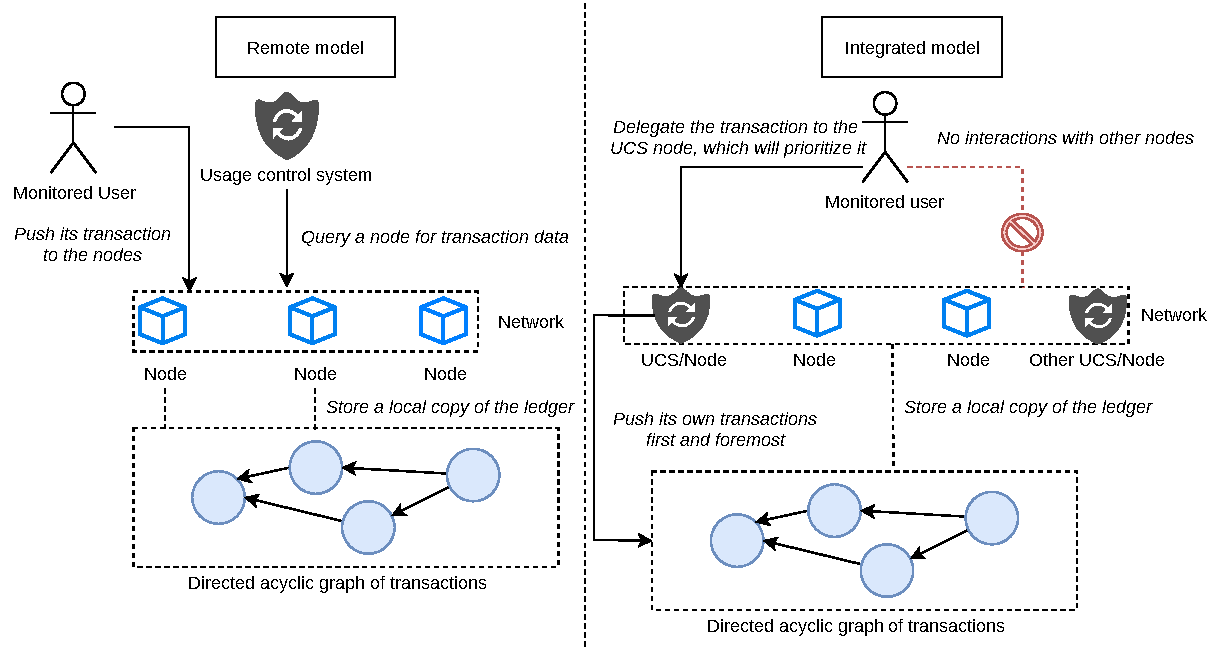
\includegraphics[width=\textwidth]{Images/remote_vs_integrated.pdf}
\caption{Differences between the remote model and the integrated model when using directed acyclic graphs.}
\label{F_peripheral_vs_integrated}
\end{figure*}

\textbf{Data management.}
For public ledgers, one key motivation for integration is the capacity to write immutable data on the ledger for transparency purposes (cf. Section~\ref{ss_integration_benefits}). Data must be classified to determine whether they can be displayed publicly or not. Data can be of four types, summarized in Table~\ref{tab:storage}: 

\begin{itemize}
    \item \emph{protected data}: data whose access is monitored by the UCS;
    \item \emph{usage control data}: data concerning the usage control, including the processes performed by the UCS as well as the results of the evaluation;
    \item \emph{users' data}: data needed by the UCS about the users, such as their attributes to make access decisions;
    \item \emph{metadata}: data about the other data, e.g., data that states the kind of processed attributes, but not the content of the attributes.
\end{itemize}

Protected data must not be stored in clear text on the ledger, and can either be encrypted on the public distributed ledger or stored in a distributed database. However, encryption produces computational overhead and the management of encryption keys is a real issue in large-scale contexts; that is why we resort to using a database management system. Usage control data describe the operations performed by the usage control system on the users. They are composed of a data identifier, the pseudonyms of the users and the action performed. They are published on the public ledger for transparency and auditability purposes. Data about users, such as their attributes, are needed only by the usage control system and are stored in the database. Finally, metadata is published on the ledger, such as timestamps and data identifiers to keep track of the data. Metadata can pose a \emph{detectability threat} when revealing its existence can lead to privacy issues, even without providing the actual content of the data, e.g., knowing the existence of a police record associated with an identity, without the content inside the record, is a sensitive information. Metadata must therefore be processed carefully, using a privacy threat analysis framework such as LINDDUN~\cite{Deng2011}.

%%%%
\begin{table}[ht] 
    \centering
    \resizebox{0.55\textwidth}{!}{%
      \begin{tabular}{|c|c|c|c|c|}
        \hline
        Data type & Data storage \\ 
        \hline
        Protected & Database \\ 
        Users' data & Database \\
        Usage control & Directed acyclic graph \\
        Metadata & Directed acyclic graph*\\
        \hline     
      \end{tabular}}
      \caption{Data types and their respective storage area \\ * If detectability is not an issue}
      \label{tab:storage}
    \end{table}  
    %%%%
\section{Performance evaluation}
\label{S_performance_evaluation}

In this section, we detail the results of a performance evaluation conducted on IOTA to demonstrate that the integration is efficient and to assess its estimated performance outcomes. To this end, we will measure the time needed for the UCS to make an access decision in the integrated setting compared to the remote node setting.

\subsection{Testbed}
\label{ss_testbed}
 \textbf{Testing environment.} To assess our contribution, we test our integration using the IOTA technology (cf. Section \ref{S_iota_dlt}). Since data are partially stored off-chain (cf. Section~\ref{ss_integration_methodology}), we relied on a \emph{Cassandra} distributed NoSQL database as decentralized storage. Cassandra is \emph{horizontally scalable}, meaning it easily handles increasing traffic demands by adding more machines~\cite{Silva2021}. Cassandra also works on low-power clusters, which is particularly suitable for the Internet of Things~\cite{Silva2021}.
 The IOTA node relies on \emph{Hornet}, a community-driven IOTA node software written in the \emph{Go} language. The usage control system is written in Java. The usage control policies are defined by the users and written using the XACML language~\cite{Godik2003}. An example of an XACML policy is provided in the appendix (Figure \ref{listing:XACML_policy}). During the tests, policies are not specified by users, but automatically derived for convenience.

\textbf{Network selection.}
IOTA has a public development network called \emph{devnet} for testing. The devnet has free tokens and is meant for testing. The public devnet could be convenient because its network is already deployed and designed to conduct tests, in particular, to measure resistance in high-load scenarios. However, it has significant drawbacks for testing. First, the network is subject to complete overhauls with no backward compatibility, preventing the reproduction of the tests conducted in our experiments on the same network. In particular, the introduction of IOTA 2.0 will lead to the removal of the IOTA 1.0 testing network. Second, the network is public, it is not possible to control the network topology including the number of nodes.

Consequently, the tests on the public network are not sufficient to ensure the efficiency of integration.
To ensure our tests can be reproduced, we deploy a \emph{private Tangle} instead. This methodology has been used by Dong \emph{et al.} \cite{Dong2019} to benchmark different DAGs including IOTA. Each node is deployed on AWS instances and constitutes a part of a private IOTA network. The network architecture of the private Tangle with AWS instances is given in Figure \ref{F_network_architecture}, for 5 nodes.

\begin{figure}[t]
\centering
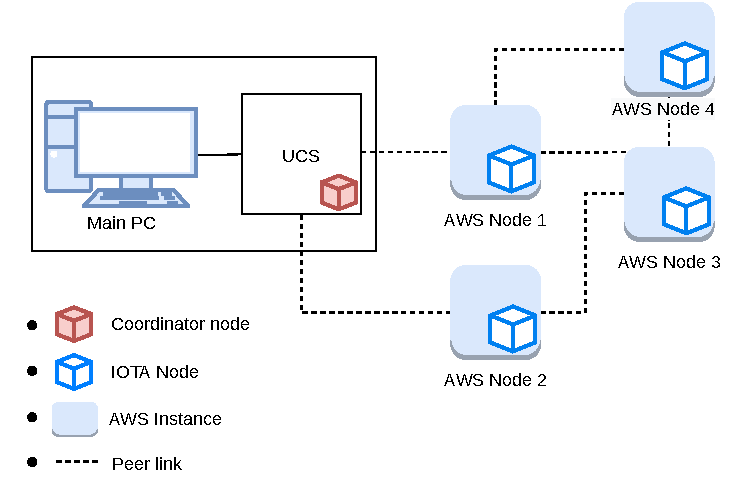
\includegraphics[width=0.8\textwidth]{Images/AWSarchitecture.pdf}
\caption{Private Tangle architecture with AWS instances - 5 nodes. Each instance runs an IOTA node, and a PC runs the Coordinator node to orchestrate the network.}
\label{F_network_architecture}
\end{figure}

\textbf{Nodes settings.} The tests are conducted using AWS t2.micro instances with 8 Gio\footnote{1 Gio=1024 Mo} storage capacity, 1 vCPU and 1 Gio RAM, consistent with the Internet of Things constraints. Another computer is used to run the usage control system, with better storage and computational power: 8Go of RAM memory, 32Go of storage and 4 CPUs. The nodes are located in Amazon's default US East (North Virginia) zone. Each Hornet node \emph{when running on the private Tangle} uses the default spammer, spamming 5 messages by second for each node. Spamming is a desired behavior, as it theoretically speeds up the transaction validation in IOTA (cf. Section \ref{S_iota_dlt}).

\subsection{Methodology}
\label{ss_methodology}

\begin{table}[h]
    \resizebox{\textwidth}{!} \\
        
        & Remote & 1020$\pm21$ ms & 85 ms & \\
        \hline
        \multirow{2}{4em}{5 nodes} & Integrated & 61$\pm3$ ms & \xmark & \multirow{2}{4em}{93.59 \%} \\
        
        & Remote & 868$\pm38$ ms & 84 ms &\\
        \hline
        \multirow{2}{4em}{7 nodes}
        
        & Integrated & 66$\pm3$ ms & \xmark & \multirow{2}{4em}{92.31 \%}  \\
        
        & Remote & 773$\pm16$ ms & 86 ms & \\
        \hline
        \multirow{2}{4em}{10 nodes}
        & Integrated & 58$\pm3$ ms & \xmark & \multirow{2}{4em}{93.77 \%}\\
        & Remote & 845 ms$\pm32 ms$ & 86 ms & \\
        \hline      
      \end{tabular}}
      \caption{Measures of transaction time (averages) for each configuration with different networks sizes}
      \label{tab:measures}
    \end{table}   

\textbf{System model.}
The agents of the system can be summarized as follows. First, the \emph{data providers} that sell data collected from their devices. Then the \emph{data buyers} pay a certain amount of cryptocurrency to be granted access to these protected data.
 The \emph{usage control system} (UCS) is responsible for monitoring the data access rights and for preventing dissemination, based on data buyers' attributes and actions. 
In particular, it processes the transactions on the \emph{distributed ledger} to grant access if the payments are duly performed. A Cassandra \emph{distributed database} shared between the data providers stores the protected data. \emph{Network nodes} validate the data buyers' transactions and propagate them to the other network nodes. The system model is depicted in Figure~\ref{F_system_model}.

\begin{figure*}[t]
\centering
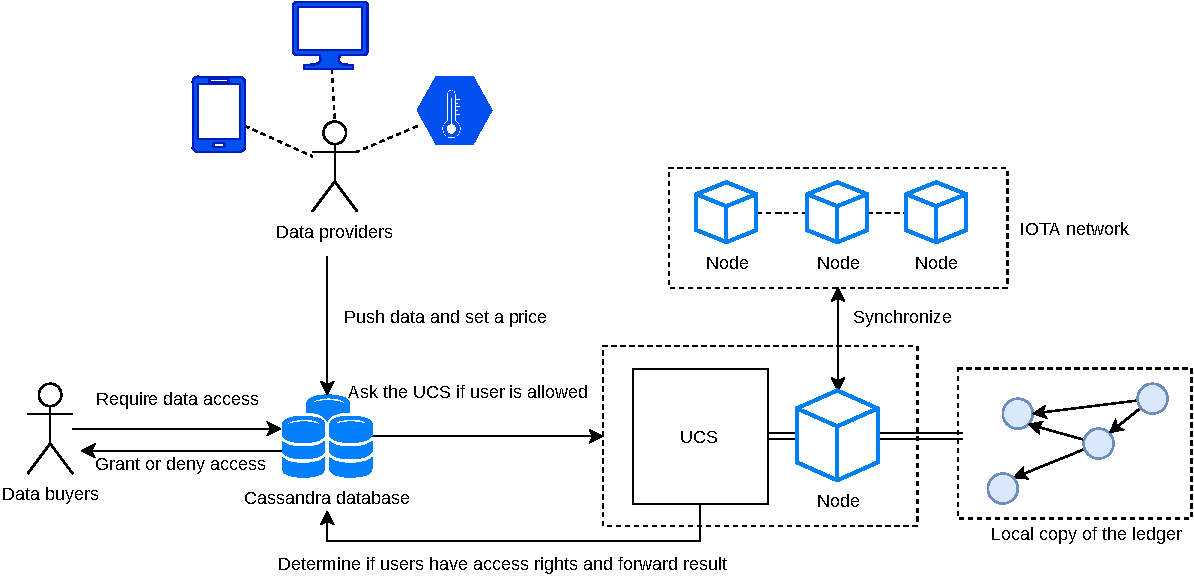
\includegraphics[width=\textwidth]{Images/system_model.pdf}
\caption{Interactions within the system model during the pre-access phase}
\label{F_system_model}
\end{figure*}

\textbf{Workflow.}
To determine which calls are of interest to assess performance outcomes of integration, the system and network calls needed for granting or denying access are detailed and classified into two categories according to the intensity of computations required,
as depicted in the sequence diagram of Figure \ref{F_sequence_iotj}. Either a call is  \emph{computationally-intensive} (1) or \emph{lightweight} (2).
This notion is comparative, such that lightweight calls are not time-consuming compared to computationally-intensive calls. 
The workflow following an access request is as follows. First, the data buyer requires access to data by sending an \texttt{accessRequest} along with its user identifier. 
Then it sends a \texttt{transaction} to an IOTA node to perform the payment. 
This node checks if the transaction is correct, e.g., no double spending, by checking it against the local state of the ledger.
If the transaction is indeed correct, the node computes a light proof of work only to prevent spam. The node then forwards the transaction to the rest of the network, using the \texttt{push} call.
The UCS then begins the monitoring of the access and sends a \texttt{requestPolicy} to its policy store, fetching the XACML policy specified by the data provider.
The UCS asks for attribute values of the data buyer (\texttt{requireAttributes}) to be able to check policy compliance. The attribute values are used for data access control, but also include values resulting from the analysis of network calls to monitor the information flow.  
When the UCS receives the attributes from the data buyer (\texttt{sendAttributes}), it fetches the transaction status on the network by calling \texttt{fetchTransaction}, then determines the policy compliance ( \texttt{checkPolicy}) to make an access decision. If the user is authorized to access the data, the UCS sends a \texttt{ grantAccess} call to the Cassandra data provider database and notifies the data buyer with a \texttt{notifyAccessResult}. Following the \texttt{grantAccess} call, the data provider sends the requested data to the data buyer with the \texttt{sendData} call.
The data buyer is monitored by the UCS for the ongoing obligations and ongoing conditions (cf. Section \ref{ss_ucon_elementaries}) with \texttt{ongoingMonitoring} calls. For convenience, only one call is represented in the sequence diagram (Figure \ref{F_sequence_iotj}),
but the monitoring usually requires numerous calls due to the continuous nature of the monitoring. The monitored data buyer must reply to \texttt{ongoingMonitoring} with \texttt{sendOngoingData} so that the UCS can make its access decisions and interrupt access if the policy is violated.
The UCS writes usage control logs and metadata for transparency on the ledger while considering privacy threats (cf. Section \ref{ss_integration_methodology} and Table \ref{tab:storage}) by calling \texttt{writeAccessLogs}. The access is finally revoked by the UCS with \texttt{revokeAccess}, should the data user request it or contravene the data provider's policy.

\begin{figure*}[ht]
\centering
 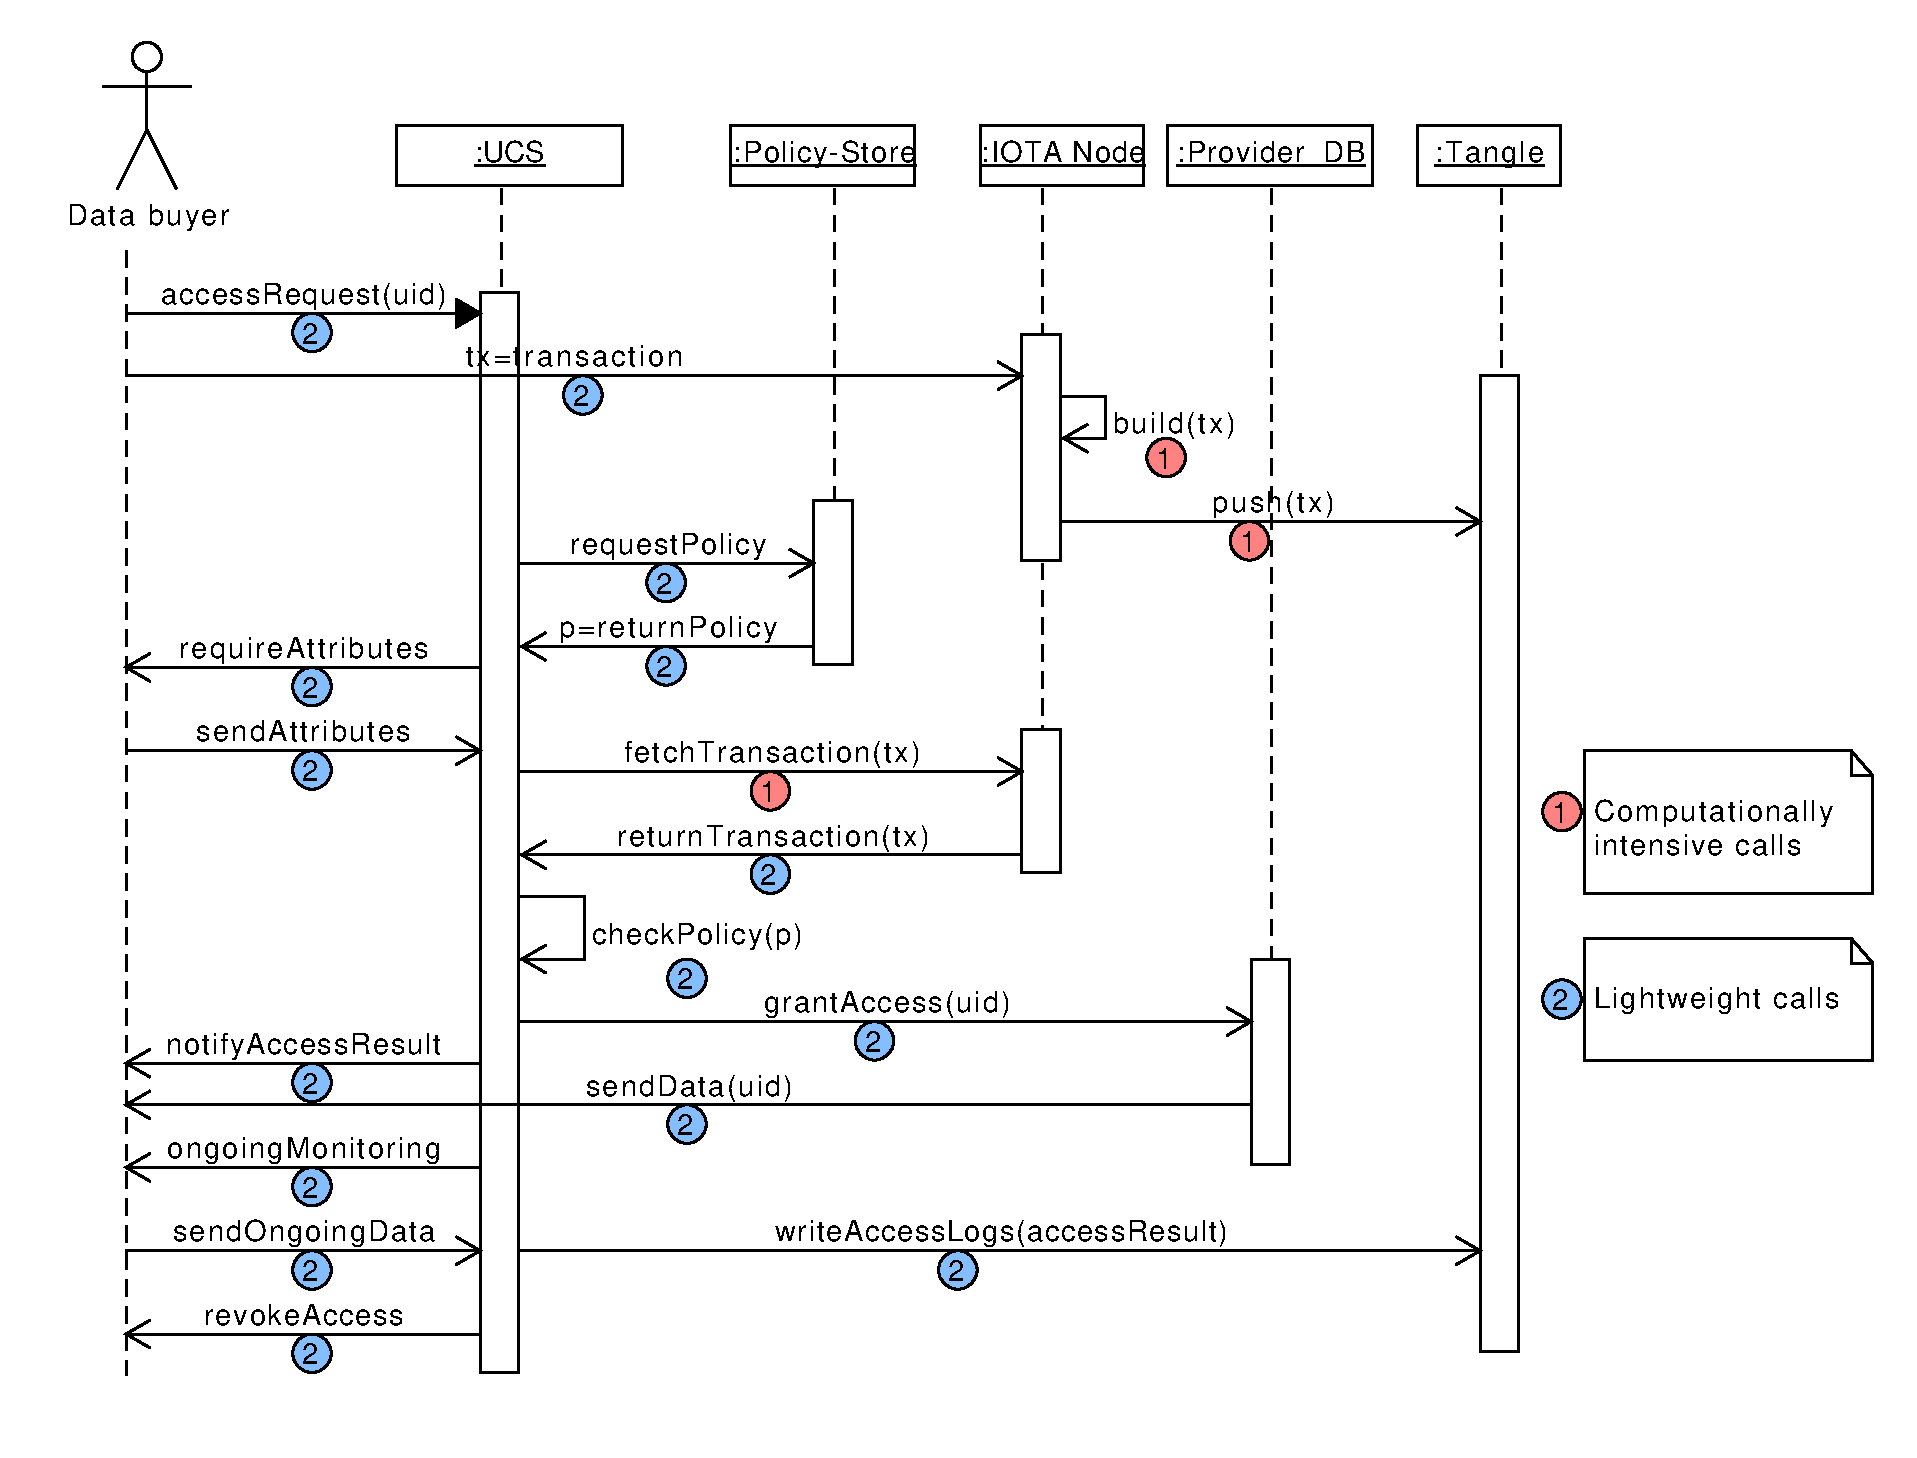
\includegraphics[width=\textwidth]{Images/sequence_iotj.pdf}
\caption{Sequence diagram for pre-access and ongoing access - UCS not integrated with IOTA}
\label{F_sequence_iotj}
\end{figure*}

\textbf{Measured calls.}
Only the \texttt{build}, \texttt{push} and \texttt{fetchTransaction} calls will be measured as the only computationally intensive calls. They are referred to as \emph{transaction time}. Our first guess would be to also include
the \texttt{checkPolicy} calls; however first tests showed that a
policy with 1000 rules takes an average 7 ms to be evaluated (1500 samples), which is lightweight compared to the transaction time. Other calls are also lightweight when measured.
The three calls \texttt{build}, \texttt{push} and \texttt{fetchTransaction} are the most time-consuming for the reasons detailed next. To build and push a transaction, the node must compute a proof of work and check that the transaction is consistent with its known ledger state.
The \emph{fetchTransaction} call is time-consuming due to several varying parameters: 1) the node is processing other transactions which delays the \texttt{fetchTransaction} call by adding it to its processing queue; 2) the (physical) distance between the node and the UCS without integration, which creates network latency; 3) the time needed to query the ledger of the node, which increases with the number of simultaneous requests.

\textbf{Transaction time.}
To demonstrate actual performance improvements, we measure the time needed for a transaction to be validated and pushed to the network, and the time required to fetch the transaction from an IOTA node. These operations are respectively the calls \texttt{build}, \texttt{push} and \texttt{fetchTransaction} of the sequence diagram of Figure \ref{F_sequence_iotj}. The \texttt{build} and \texttt{push} calls are grouped under a single API call in the Java IOTA library and correspond to only one common measure.
Tests are conducted in the two different configurations, respectively the remote and the integrated settings: (1) the UCS interacts with a remote IOTA node running in an AWS instance; (2) an integrated node that runs both the UCS and an IOTA node concurrently, as illustrated in Figure \ref{F_peripheral_vs_integrated}.
For each test, 1500 samples ($N=1500$) are used and confidence intervals are given with a 95\% confidence level.

\subsection{Results}
\label{ss_results}

The results of experimental measurements are summarized in Table~\ref{tab:measures}. For convenience, only the experiments with 5 nodes $N=5$ are first discussed. We then detail the impact of the number of nodes on the results and provide further explanations.

\textbf{Remote setting}. When the UCS interacts with a remote node, the \texttt{build} and \texttt{push} calls need an average $\overline{t}_{transaction, r} =868\pm 31 ms$ with 5 nodes in the network. Building and pushing a transaction requires a minimum $m_{r}=646 ms$ and a maximum $M_{r}=7649 ms$. This wide range is caused by nodes which are often desynchronized and have to update the state of the ledger before pushing their transactions. 
Additionally, the UCS has to recover the result of the transaction requiring an additional $\overline{t}_{fetch, r} = 84\pm0.38ms$.

\textbf{Integrated setting}. When using an integrated node on the UCS device, the transaction time improvements are significant. Indeed, the \texttt{fetchTransaction} call does not involve any network calls and requires less than 1 ms to be completed when measured. Our own transactions are prioritized on our node, substantially decreasing the time to complete the \texttt{build} call. The average time needed to \texttt{build} and \texttt{push} a transaction drops to $\overline{t}_{transaction, l}=61\pm2.86ms$.

\textbf{Number of nodes.} As the number of nodes increases, the impact of integration in percentage remains steady, varying from a 92.31\% to a 94.12\% transaction time decrease. The transaction time in our integration scheme is consequently 13 to 18 times faster compared to the remote node setting.

The time required to build and push transactions decreases before 7 nodes, then starts to go up when using 10 nodes. Firstly, the number of messages spammed increases with the number of nodes. We can therefore observe the expected behavior of IOTA \cite{Popov2017}: as the number of transactions per second increases, transactions are validated faster. Secondly, when reaching 10 nodes, there are approximately 50 messages spammed per second as each node spams 5 messages per second. There are two possible explanations for this behavior. First, the network could saturate due to the Coordinator milestones validation.
This issue is well-identified by both the IOTA foundation and academics \cite{Conti2022, Wang2022} and is the motivation for the development of IOTA 2.0, willing to remove the Coordinator. However, the Coordinator runs on the same device in both integrated and remote settings, but the transaction time does not increase for 10 nodes in the integrated setting. Therefore, we can conclude that it is not the Coordinator that saturates, but the remote node used for the testing. Indeed, the nodes running on AWS are resource-constrained, and processing 50 transactions per second is time-consuming for an instance with 1 Gio of RAM and 1 vCPU.

\section{Privacy evaluation}
\label{S_privacy_evaluation}
 In this section, we conduct a privacy threat analysis, to highlight the risks for the users either selling or buying data in the system as described in Section \ref{ss_methodology}. Based on this analysis, we then detail how usage control mitigates the different privacy risks.

\subsection{Threat model} The \emph{usage control system} is considered \emph{honest-but-curious}. It fulfills its usage control tasks but may be interested in collecting undue data about the users it monitors. This behavior may be financially motivated, i.e., to sell the users' data afterward. In particular, the UCS has an interest in gathering the system calls and network calls of the monitored users, both carrying valuable, privacy-sensitive data.

\emph{Data buyers} and \emph{data providers} are considered honest-but-curious as well. Notably, data buyers try to infer more data from the protected data they buy, but do not try to bypass the UCS monitoring or to compromise the database.
The \emph{Cassandra distributed database} is considered as trusted and not compromised.

\subsection{Privacy risks}
\label{ss_privacy_risks}

 The \emph{LINDDUN privacy threat modeling framework} \cite{Deng2011} (cf. Section \ref{ss_privacy_threat_modeling}) is used to describe the 
 different privacy risks faced by data buyers and data renters.
\textbf{Items of interest.} Items of interest (IOI) in LINDDUN refer to any data element, including users' personal data or transaction data, that is considered privacy-sensitive. It is paramount to exhaustively identify which items are of interest before conducting the privacy threat assessment, to ensure the full listing of the threats. Items of interest can be subjects, messages, actions or data. \sul{In scenarios involving transactions, the items of interest can be}:
\begin{itemize}
    \item the geolocated protected data generated by data providers;
    \item the transaction data, including but not limited to users' addresses and transaction values;
    \item users' data, i.e., data buyer and data provider personal data;
    \item usage control data, such as the results of access requests;
    \item metadata, such as the time the data was created or added to the Cassandra database, that can be used to infer other data.
    \item data buyers, data providers, the UCS and the Cassandra database, i.e, subjects;
    \item network messages between the subjects, and the messages between the UCS components (cf. Section \ref{ss_ucon_architecture});
    \item actions carried out by the subjects, such as an access request by the data buyer, entry insertion on the database by the data provider or the beginning of an access request evaluation by the UCS.
\end{itemize}

In the following, transaction data are ignored, as preserving privacy in distributed ledgers is a specific, orthogonal research topic. Legal compliance in particular is troublesome for distributed ledgers \cite{Haque2021}, and privacy-enhancing technologies have been designed to address privacy threats, such as cryptocurrency mixers for linkability \cite{Sarfraz2019}, \cite{Glaeser2022}.


\textbf{Linking (L).} Linking occurs when two \emph{items of interest} are associated to learn more about an individual or a group. Due to the diversity of agents and technologies involved, linking threats are numerous in the electricity consumption prediction scenario:

\begin{enumerate}
    \item linkage between protected data and its owner (user data). The location in the protected data can be used to facilitate the re-identification of the data providers (I);
    \item linkage between a data buyer and a data provider. It simplifies re-identification when one of them is identified (I);
    \item linkage between metadata and usage control data, as both are written on the ledger.
\end{enumerate}

Linking leads to other identifying (I), detection (D) and non-repudiation (N) threats and is triggered by data disclosure (D) - the more data available, the more likely are linking threats.

\textbf{Identifying (I).} Identification is occurring when an attacker learns the identity of an individual, breaking its anonymity or pseudonymity. This threat distinguishes \emph{identified data} where the identity is explicitly maintained, and \emph{identifiable data} which enables to derive the identity indirectly. Users' attributes, e.g., IP address or processed by the usage control system to make an access decision can be used to infer the user's true identity. In the scenario, the risks are to re-identify data buyers and data providers, using protected data, usage control data or metadata.

\textbf{Non-repudiation (N).} Non-repudiation, in LINDDUN privacy threat assessment, is the ability to attribute a claim to an individual. For example, the impossibility for a data buyer to deny they bought and accessed protected data, or for data providers to deny they generated a given data, are non-repudiation threats.

\textbf{Detecting (D).} Detecting is the ability to deduce the involvement of an individual in an action with observation. Detecting does not require being able to read the actual data. Knowing that the data exists is enough to infer more sensitive information. Detecting can be done by observing \emph{communications} or \emph{application side-effects}. Detecting threats in the electricity consumption prediction scenario includes: 
\begin{enumerate}
    \item detecting that a user is monitored by analyzing the communications of the UCS. An attacker learns that the user has likely bought valuable data;
    \item detecting what are the protected data and where they are disseminated, without the actual content of the data, by analyzing the UCS logs;
    \item detecting users' attributes by intercepting the communications between the policy information points (PIP) and the context handler (CH) (cf. Section \ref{ss_ucon_architecture});
\end{enumerate}

\textbf{Data disclosure (D).} Data disclosure is the
immoderate collecting, storing, processing or sharing of personal data. This generic threat focuses on four characteristics:
\begin{enumerate}
    \item \emph{unnecessary data types}, if the data granularity or sensitivity is too detailed;
    \item \emph{excessive data volume}, if the amount or the frequency of data processing is too high;
    \item \emph{unnecessary processing}, if the data is processed or disseminated out of necessity;
    \item \emph{excessive exposure}, refers to how widely accessible the data is and to whom the data is shared.
\end{enumerate}

In the energy consumption prediction scenario, data disclosure can occur if a data provider has access to protected data while not fulfilling the policy's conditions, or can disseminate it outside of the UCS monitoring perimeter. Similarly, data disclosure occurs if the UCS collects too detailed data about the data buyers to monitor them.

\textbf{Unawareness (U).} Unawareness occurs when an individual is insufficiently informed and involved in the processing of personal data.
Unawareness occurs in the scenario if the data providers are not informed about the privacy threats they face by
selling their data with associated geolocation. The user may also be unaware of the privacy risks of accepting to be monitored by the UCS, which writes usage control data on the ledger, that are potentially privacy-sensitive (cf. Section \ref{ss_methodology}) 

\textbf{Non-compliance (N).} Non-compliance is the deviation from security and data management best practices, standards and legislation. This risk occurs if the processing of any item of interest is considered unlawful based on the specified policies and the applicable regulations, e.g., GDPR \cite{EUdataregulations2018}. In the scenario, the risks are that although the data provider specifies a policy, it is not properly enforced by the usage control system.
% In particular, users lack \emph{intervenability} in the scenario: once the transaction data
% are written on the ledger, they can not be removed. This is a common issue in distributed ledger, contravening GDPR's articles 16 and 17 - right to rectification and erasure} \cite{EUdataregulations2018}.

% \ul{Another issue is the data \emph{retention time}, which should be limited to the time required to process the data. Yet, the data written on the ledger, i.e., usage control data and some metadata, are stored indefinitely. Besides, the principle of data minimization (article 5)}\cite{EUdataregulations2018} \ul{ requires that only the necessary data be collected and processed. However, in a public distributed ledger like IOTA, all participants have access to all data, including unnecessary or irrelevant data. The GDPR also requires that data controllers and processors ensure the protection of personal data (Article 32)}\cite{EUdataregulations2018} \ul{. Using IOTA, users push the transactions themselves. It is hard to determine who is responsible for compliance. Finally, consent may not be possible or practical (Article 7)}\cite{EUdataregulations2018} \ul{, as anyone can access the data on the ledger without the need for consent}

\begin{table}[ht] 
    \resizebox{\textwidth}{!}{%
      \begin{tabular}{|c|c|c|c|c|}
        \hline
        Threat & Scenario example & Mitigated by the UCS\\
        \hline
        Linking & Link between data owner and buyer & ?\\
        Identifying & Data provider is re-identified & ?\\
        Non-repudiation & Data provider can not deny data generation & \xmark \\
        Detecting & Detect a user is monitored & \cmark\\
        Data disclosure & Protected data dissemination & \cmark\\
        Unawareness & Inference risks of location unknown  & \cmark\\
        Non-compliance & Data provider policy not enforced & \cmark\\
        \hline      
      \end{tabular}}
      \caption{LINDDUN privacy threat analysis, based on the illustrative scenario.\\ (?) marks 
means the threat is only partly mitigated by the UCS.}
    \label{tab:threats}
    \end{table}   

\subsection{Threat mitigation with usage control}
\label{ss_mitigation}

As a privacy-enhancing technology, usage control is designed to address a significant part of the above-mentioned privacy threats. We next detail how these threats are addressed, and which ones can not be mitigated by the UCS. The results are summarized in Table \ref{tab:threats}.


\textbf{Linkability. (?)}
The usage control system has only a partial impact in preventing this threat. Notably, the linkage between metadata and usage control data, which are both unrestricted data available publicly on the ledger, can be accessed without monitoring in the first place. However, the UCS monitors the dissemination and the processing of the protected data, limiting the risks to link them to their owners.

\textbf{Identifying. (?)} Similarly, the usage control system must be able to identify the data buyer to fulfill its mission. While it can prevent users from disclosing \emph{identified data}, it is much harder for it to prevent inference from \emph{identifiable data}.

\textbf{Non-repudiation. \xmark}  To fulfill its task, the UCS needs to ensure that a monitored data buyer can not decline having disseminated the data, or having processed it in an unlawful manner. Therefore, the UCS not only does not guarantee non-repudiation, but also writes usage control data on the distributed ledger, making non-repudiation impossible.

\textbf{Detecting. \cmark} To mitigate this threat, all communications are secured using TLS, notably the communication between the usage control system and the users, the context handler and the PIPs, as well as the context handler and the PEPs. Besides, unless the UCS is compromised, an attacker does not have access to the logs of the UCS.

\textbf{Data disclosure. \cmark} The data processing is monitored by the usage control system, mitigating the \emph{excessive data volume} threat. The usage control system, by monitoring both the information flow and the usage of the data, also prevents \emph{unnecessary processing}. \emph{Excessive exposure} is prevented as part of the access control to the data.

\textbf{Unawareness. \cmark} The usage control system asks data owners to design data policies themselves, directly addressing the unawareness threat.

\textbf{Non-compliance. \cmark} The usage control system monitors the data buyers, stopping them from processing the data unlawfully. The usage control system, considered honest-but-curious, enforces the proper usage control policy specified by the data provider.


Usage control addresses four categories of threats directly, i.e., detecting, data disclosure, unawareness and non-compliance. Due to the diversity of the data and agents considered, linking and identifying threats are only partially mitigated. Only the non-repudiation threat is not considered by usage control.

\section{Conclusion}
\label{S_conclusion_integration}

In this chapter, we introduced and evaluated the integration of usage control with distributed ledger technologies. After identifying the 
possible compatible DLTs (Section \ref{ss_integrability_criteria}), we developed a proof of concept using IOTA before conducting performance tests (Section \ref{S_performance_evaluation}).
\sul{Even though similar works exist in the state of the art that propose the integration (also referred to as incorporation) of usage control with blockchains, the integration is always conducted in private blockchain settings. 
The work in this thesis therefore comes as a novelty, by studying the integration process itself, and by identifying DAG-based distributed ledgers as 
potential permissionless solutions for large-scale IoT networks.} 

While this chapter focused on usage control, the integration principle can be generalized to any system that requires to process
distributed ledger transactions and that can be deployed on a node. 
The network security always benefits from having more nodes (cf. Section \ref{ss_integration_benefits}).
For example, the mixing services can benefit from integration (cf. Section \ref{ss_obfuscation_coin_mixing_merge_avoidance}), especially
when decentralized as used in Chapter \ref{C_solving_trilemma} as the mixing peers can be numerous. 
Similarly, a device will benefit from deploying a node if it has to analyze the transaction, which is the case for the UCS so as to monitor access. In the next Chapter \ref{C_formalism}, we will digress from practical optimization aspects and discuss modeling. We will see the limitations of the current usage control formalism and how it can be better adapted to the Internet of Things.  